%\pdfoutput=1
\documentclass[11pt]{article}

\usepackage[table,xcdraw]{xcolor}
% \usepackage{ACL2023}
\usepackage{amsmath}
\usepackage{latexsym}
\usepackage[T1]{fontenc}

\usepackage[utf8]{inputenc}
\usepackage{fancyhdr}
\usepackage{graphicx}
\usepackage{float}
\usepackage{subfig}
\usepackage{booktabs}
\usepackage{url}


%%%%%%%%%%%%%%%%%%% TITLE AND AUTHORS %%%%%%%%%%%%%%%%%%%

\title{IIC3633  Análisis \& Baselines proyecto de Recomendación multimodal de juegos de mesa}

\author{\normalfont 
Eduardo Salinas | 21624453 | \texttt{esalinasbarros@uc.cl} \\
Nicolás Gutiérrez | 20203772 | \texttt{njgutierrez@uc.cl} \\
Alfonso Badilla | 20640854 | \texttt{alfonso.badilla@uc.cl} \\
% comment line below if only 3 team members
%Author 4 | SCIPER 4 | \texttt{author4@epfl.ch} \\
}

%%%%%%%%%%%%%%%%%%% PROPOSAL %%%%%%%%%%%%%%%%%%%

\begin{document}
\maketitle
\newpage

\section{Descripción del problema y justificación}
Actualmente, el mercado de los juegos de mesa esta experimentando un crecimiento significativo, lo que implica una gran cantidad de juegos nuevos en el mercado cada día con una alta variedad de generas, temas y niveles de complejidad. Aunque existen clasificadores generales con reseñas, esto no toma en consideración los gustos personales. 

Un sistema recomendador que sea capaz de recomendar juegos según fotos, descripciones sobre aspectos del juego, lenguaje natural e historial de gustos le da un aspecto de personalización al problema, mejorando la solución significativamente y potenciando la toma de decisiones a la hora de elegir un juego de mesa que encaje con lo esperado por el usuario. Además, dado el gran crecimiento del mercado de juegos un sistema como el explicado, sera cada vez mas utilizado y explotado para elegir juegos de calidad.

\section{Objetivos del proyecto}
El objetivo del proyecto es crear un sistema recomendador de juegos de mesa, que sea capaz de hacer las recomendaciones en base a imágenes y características descriptivas (metadata) utilizando filtrado colaborativo. La idea es que el sistema sea multimodal y que pueda recibir diferentes formatos de datos de entrada para dar recomendaciones validas que al usuario le gustaran. Para esto, se utilizaran métricas de testeo de sistemas recomendadores como precisión, novelty y diversidad.

\section{Analisis descriptivo de los datos}
El dataset que se utilizara para este proyecto consta de 10 archivos diferentes, cada uno con información diferente sobre juegos de mesa. El punto de entrada sera el archivo \texttt{user\_ratings.csv} el cual consiste de 19 millones de filas. Por temas de procesamiento limitado de Google Collab, se utilizaran 50.000 filas para el entrenamiento  inicial. A continuación ser presenta un desglose de los diferentes archivos a utilizar:

\begin{itemize}
    \item \texttt{games.csv}: Este archivo contiene 22 atributos sobre los juegos calificados y contiene 22.000 juegos diferentes. Entre los atributos tenemos aspectos como la descripción del juego, que se podrían evaluar usando modelos de lenguaje, el año de publicación (que distribuye como se muestra en la figura \ref{fig:publishYear}), el rating promedio recibido, entre otros.
    \item \texttt{ratings\_distribution.csv}: Contiene el total de ratings en cada juego de mesa. En general estos ratings distribuyen como se ve en la figura \ref{fig:distribucionRatings}.
    \item \texttt{temes.csv}: Contiene las temáticas de cada juego como un flag binario. Las 50 más comunes se pueden ver en el gráfico de la figura \ref{fig:tematicasComunes}.
    \item \texttt{mechanics.csv}: Contiene las mecánicas del juego como un flag binario. Las 50 más comunes se pueden ver en el gráfico de la figura \ref{fig:mecanicasComunes}.
    \item \texttt{subcategories.csv}: Contiene las subcategorías de cada juego en formato flag binario.
    \item \texttt{artists\_reduced.csv}: Contiene la información sobre que artista creo cierto juego en formato flag binario. Solo se consideran artistas con mas de 3 juegos creados.
    \item \texttt{designer\_reduced.csv}: Contiene la información sobre que diseñador diseño cierto juego en formato flag binario. Solo se consideran diseñadores con mas de 3 juegos creados.
    \item \texttt{publishers\_reduced.csv}: Contiene la información de las empresas que venden dichos juegos en formato flag binario. Solo se consideran las empresas que veden mas de 3 juegos.
    
\end{itemize}

\begin{figure}
    \centering
    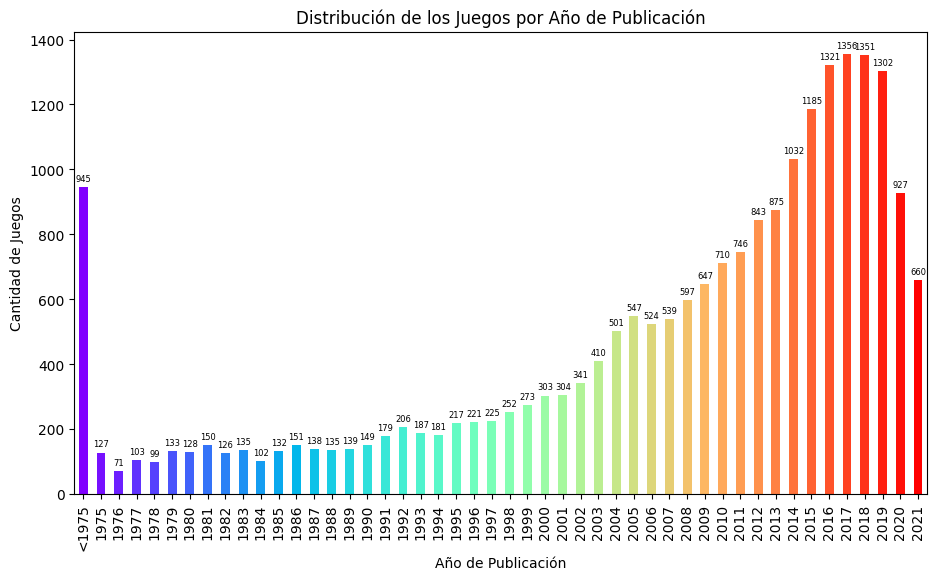
\includegraphics[width=0.8\linewidth]{publishYear.png}
    \caption{Juegos por año de publicación}
    \label{fig:publishYear}
\end{figure}

\begin{figure}[h]
    \centering
    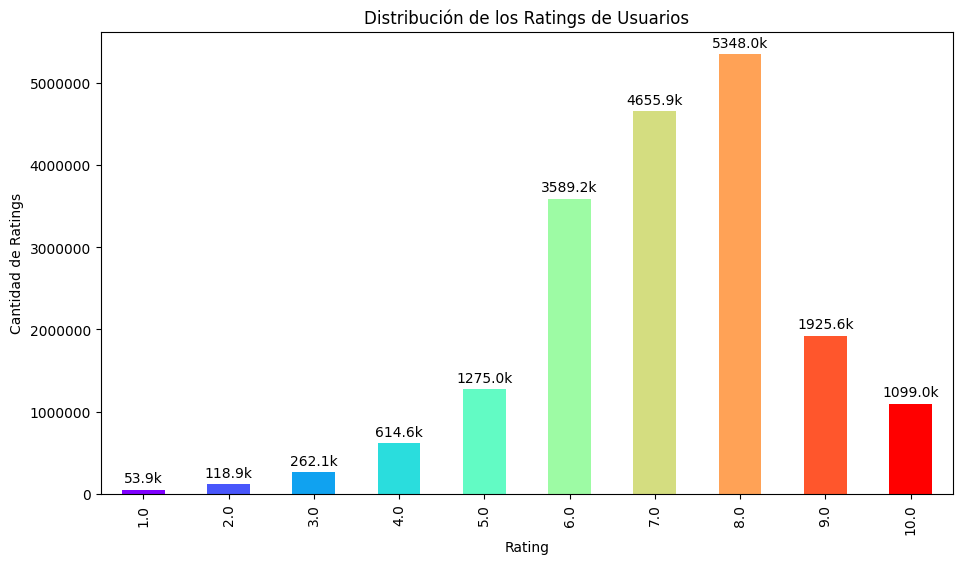
\includegraphics[width=0.8\linewidth]{distribucionRatings.png}
    \caption{Distribución de ratings de juegos}
    \label{fig:distribucionRatings}
\end{figure}

\begin{figure}[h]
    \centering
    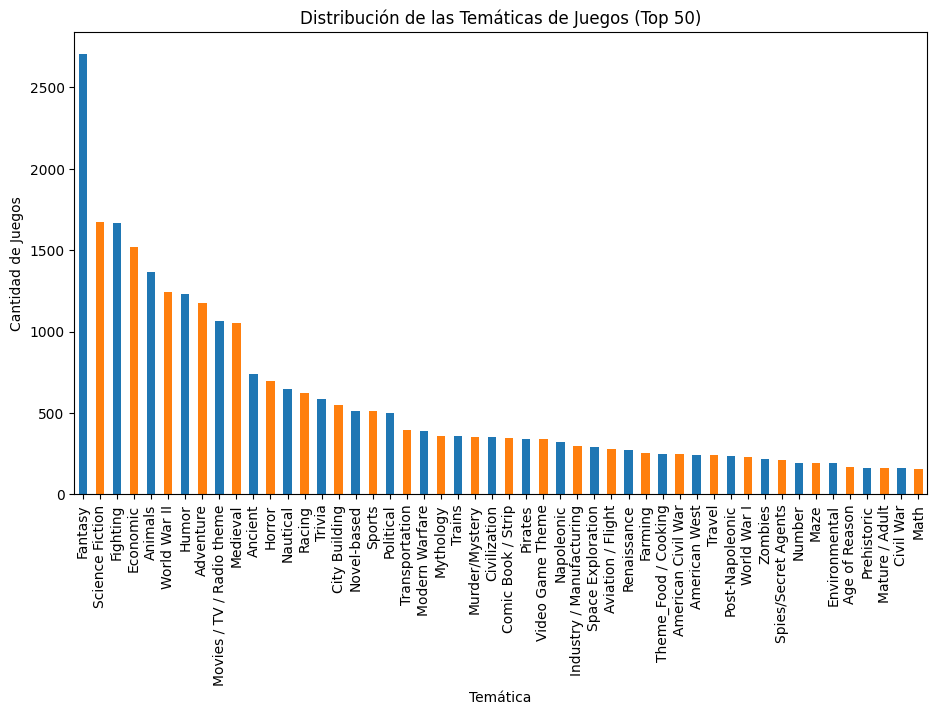
\includegraphics[width=0.8\linewidth]{tematicasComunes.png}
    \caption{Temáticas más comunes en el dataset}
    \label{fig:tematicasComunes}
\end{figure}

\begin{figure}[h]
    \centering
    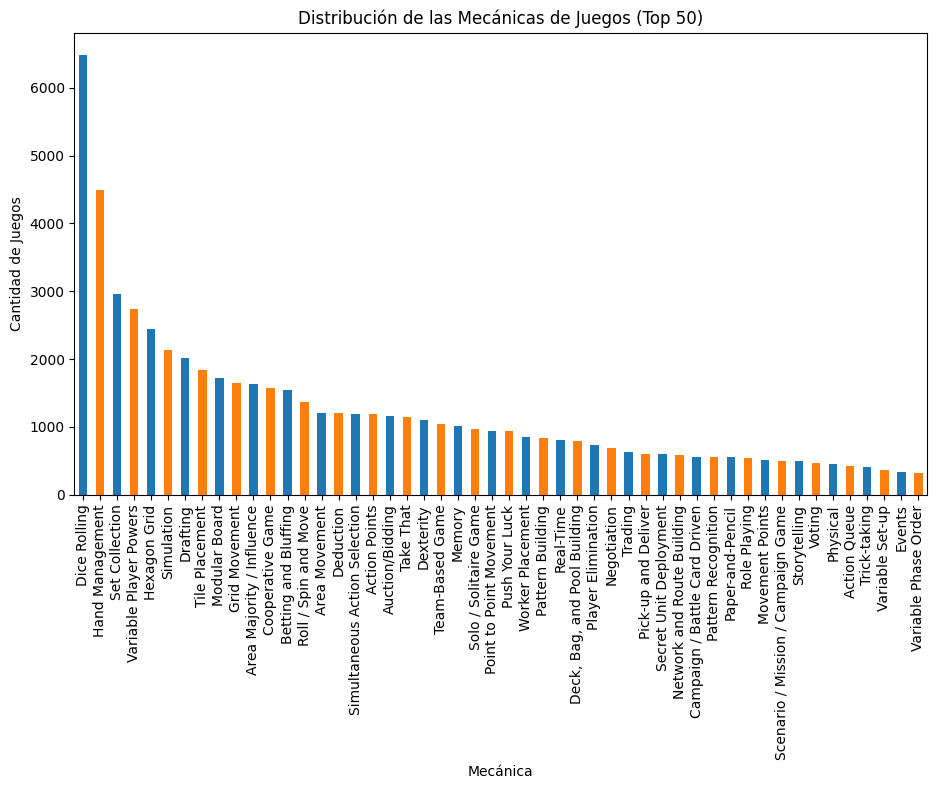
\includegraphics[width=0.8\linewidth]{mecanicasComunes.png}
    \caption{Mecánicas más comunes en el dataset}
    \label{fig:mecanicasComunes}
\end{figure}

\section{Implementación de modelos de referencia} 
Para tener una idea basica de las metricas de recomendación actuales, entrenamos 4 modelos y obtuvimos las siguientes metricas.
\begin{table}[h!]
\centering
\begin{tabular}{|l|c|c|c|c|}
\hline
\textbf{Modelo}    & \textbf{MAE}   & \textbf{RMSE}  & \textbf{MAP}     & \textbf{NDCG}        \\ \hline
ItemKNN            & 7.1102         & 7.1102         & 1.15e-4          & 5.873e-5             \\ \hline
SVD                & 7.2539         & 7.2539         & 1.54e-4          & 5.873e-5             \\ \hline
MostPopular        & -              & -              & 0.077            & 0.057                \\ \hline
Random             & 2.827          & 3.45           & -                & -                    \\ \hline
\end{tabular}
\caption{Resultados de diferentes modelos de recomendación}
\end{table}
\newline
Se pueden observar errores relativamente altos para los modelos ItemKNN y SVD y metricas de precision bastante bajas. Los otros algoritmos tampoco están mostrando un desempeño muy alto, lo que hace referencia a una falta de calidad en el dataset. Dicho esto, si bien hay una falta de metricas, se puede observar que MostPopular y Random funcionan mejor que ItemKNN y SVD.




\section{Planificación para la etapa Midterm} 
El trabajo que realizaremos se espera que se distribuya en dos partes:
\begin{enumerate}
    \item \textbf{Aprovechar metadata cualitativo:} Primero se hará una comparación de los modelos de baseline con uno que incorpore el metadata de las tablas adicionales del dataset entregado, y se verá si se logra ganancia de precisión y otras métricas considerando ese metadata. Se espera tener esto listo entre la segunda y tercera entrega, con al menos un avance en la segunda, y se debería evaluar en función de la robustez de la utilización del metadata relevante para entrenar modelos, es decir si se utilizó el metadata de una cantidad de formas suficientes para entrenar un modelo suficientemente bueno.
    \item \textbf{Aprovechar imágenes y descripción de los juegos:} Luego se repetirá este experimento pero agregando además como metadata las imágenes y la descripción relacionados con los respectivos juegos de mesa, considerando también performance en tiempo del modelo, para revisar si se obtiene ganancia suficiente de considerar estos datos dentro del metadata cualitativo del modelo (se agragecería feedback especialmente en la factibilidad y forma de hacer esta parte del trabajo). Si se realizara, se haría para la tercera entrega, y se debería evaluar en función de la profundidad de la investigación relacionada con la aplicación de estas formas de metadata.
\end{enumerate}


\section{Bibliografía relevante}

\begin{itemize}
    \item En el artículo "Addressing the user cold start with cross-domain collaborative filtering: exploiting item metadata in matrix factorization" \url{https://link.springer.com/article/10.1007/s11257-018-9217-6} se utiliza filtrado colaborativo y se busca reducir el efecto del "cold start" de un usuario nuevo utilizando el metadata de los ítems de la plataforma.
    \item En el artículo "Using geospatial metadata to boost collaborative filtering" \url{https://dl.acm.org/doi/abs/10.1145/2507157.2507201} se utiliza metadata de espacio para recomendar ítems del tipo fotos junto con filtrado colaborativo.
\end{itemize}


\end{document}


